\documentclass{standalone}
\usepackage{tikz}
\usetikzlibrary{calc}
\begin{document}
	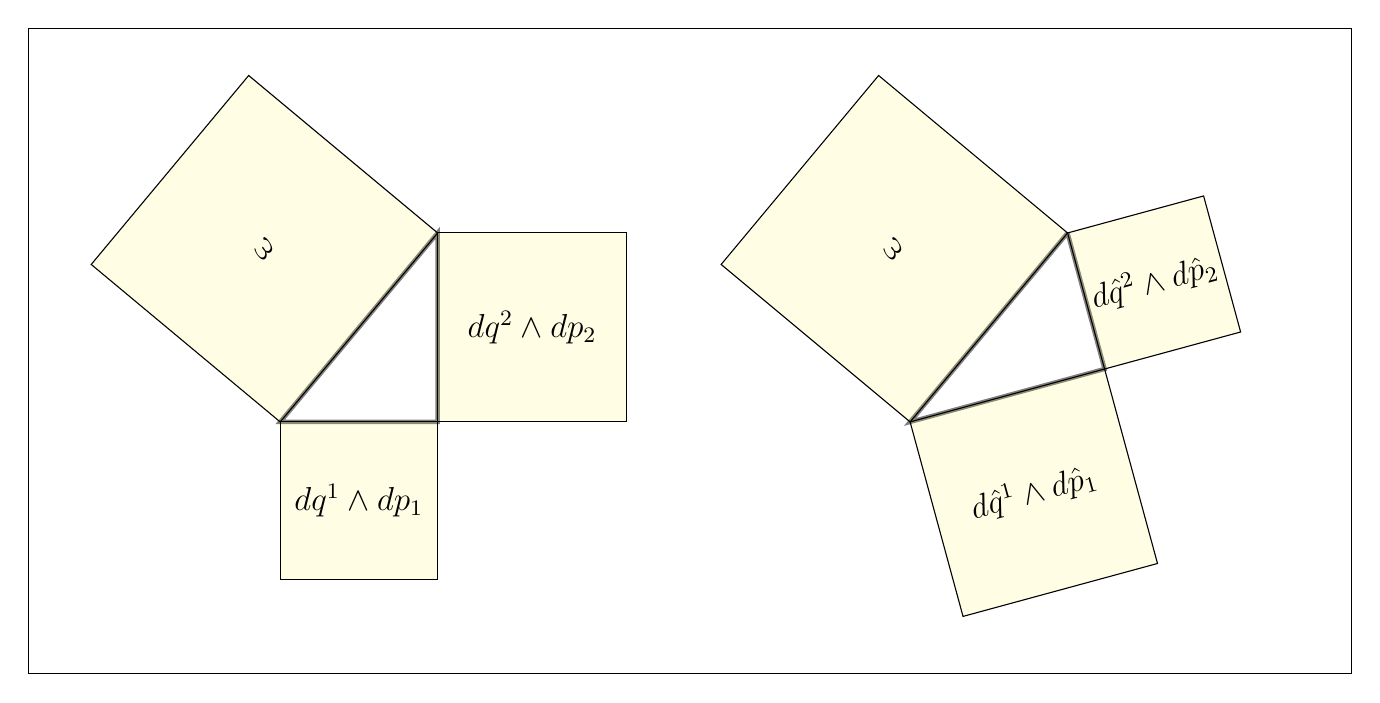
\begin{tikzpicture}[scale=.4]
	
	% INPUTS
	
	\newcommand{\xvar}{5};					% x component of omega
	\newcommand{\yvar}{6};					% y component of omega	
	\newcommand{\xprimevar}{6.4};	    % length of the bottom side of the second triangle, called x prime
	% Note: must have  x' < omega = sqrt(x^2 + y^2) 
	
	\newcommand{\dvar}{20}; 				% space between the two drawings
	
	% outer rectangle and diagram name
	\draw (-8,-8) rectangle (34,12.5);
	
	% outer rectangle and diagram name, alternate method, needs more calculations...
	%		\draw (-\yvar - 2,-12) rectangle (\dvar + \dvar, \yvar + \xvar + 2);
	%		\node at (13,-8) {\huge Independent d.o.f.};
	
	% calculate omega from x and y components
	\newcommand{\omegalength}{sqrt(\xvar*\xvar+\yvar*\yvar)}
	
	% calculate the angle that omega creates w.r.t. the horizontal axis
	\newcommand{\thetavar}{atan2(\yvar,\xvar)}
	
	\newcommand{\yprimevar}{sqrt(\omegalength*\omegalength - \xprimevar*\xprimevar)}
	
	\newcommand{\thetaprimevar}{atan2(\yprimevar,\xprimevar)}
	
	
	% calculations
	\newcommand{\phivar}{90-\thetavar};							  % second angle 
	\newcommand{\phiprimevar}{90-\thetaprimevar};	 	   % second prime angle
	
	% styles
	\tikzstyle{triangle}=[ultra thick,fill=white,opacity=0.5];
	\tikzstyle{projection} = [fill=yellow,fill opacity=0.1,text opacity =1,text=black];
	
	% drawing the right basic triangle 
	\filldraw[style=triangle] (0,0) -- (\xvar,0) -- (\xvar,\yvar) -- cycle;
	
	\filldraw[style=projection] (0,0) rectangle (\xvar,-\xvar) node[pos=.5] {\large $ {dq^1}\wedge {dp_1}$};
	
	\filldraw[style=projection] (\xvar,0) rectangle (\xvar + \yvar, \yvar) node[pos=.5] {\large ${dq^2}\wedge {dp_2}$};
	
	\filldraw[style=projection,rotate around={\thetavar:(0,0)}]  (0,0) rectangle ({\omegalength}, {\omegalength}) node[pos=.5, rotate={\thetavar}] {\large $\omega$};
	
	% drawing the complex right triangle  
	\filldraw[style=triangle,rotate around={\thetavar:(\dvar,0)}] ({\dvar + \omegalength},0) -- ({\dvar},0) -- ++({-\thetaprimevar}: {\xprimevar}) -- ++({\phiprimevar}:{\yprimevar});
	
	\filldraw[style=projection,rotate around={\thetavar - \thetaprimevar:(\dvar,0)}]  (\dvar,0) rectangle (\dvar + \xprimevar,-\xprimevar) node[pos=.5, rotate=\thetavar-\thetaprimevar] {\large $d\hat{q}^1\wedge d\hat{p}_1$};
	
	\filldraw[style=projection,rotate around={\thetavar - \thetaprimevar:(\dvar,0)}]  ({\dvar + \xprimevar},0) rectangle ({\dvar + \xprimevar + \yprimevar}, {\yprimevar}) node[pos=.5, rotate={\thetavar-\thetaprimevar}] {\large $d\hat{q}^2\wedge d\hat{p}_2$};
	
	\filldraw[style=projection,rotate around={\thetavar:(\dvar,0)}]  (\dvar,0) rectangle ({\dvar + \omegalength}, {\omegalength}) node[pos=.5, rotate=\thetavar] {\large $\omega$};		
	
	
	\end{tikzpicture}

\end{document}